%%%%%%%%%%%%%%%%%%%%%%%%%%%%%%%%%%%%%%%%%%%%%%%%%%%%%%%%%%%%%%%%%%%%%%%%
%  First draft.  Springer proceedings class (svproc), not tied to any
%  particular conference.  Every number is generated by the code of this
%  repository; paper/README.md says where each one comes from.
%%%%%%%%%%%%%%%%%%%%%%%%%%%%%%%%%%%%%%%%%%%%%%%%%%%%%%%%%%%%%%%%%%%%%%%%
\documentclass{svproc}

\usepackage{url}
\def\UrlFont{\rmfamily}
\usepackage{amsmath,amssymb}
\usepackage{graphicx}
\usepackage{booktabs}
\usepackage{multirow}
\usepackage{algorithm}
\usepackage{algpseudocode}

\newcommand{\mcal}[1]{\mathcal{#1}}
\newcommand{\ITAE}{\mathrm{ITAE}}
\newcommand{\MSE}{\mathrm{MSE}}

\begin{document}
\mainmatter

\title{Torque-Aware Tuning of Fractional-Order PID Controllers for a Six-Degree-of-Freedom
Robotic Arm with a Fractional-Order PSO--Grey Wolf Hybrid}
\titlerunning{Torque-Aware FOPID Tuning with FOPSO-GWO}

% TODO: authors, affiliations and e-mail addresses
\author{First Author\inst{1} \and Second Author\inst{2}}
\authorrunning{F. Author and S. Author}
\institute{Department, Institution, City, Country,\\
\email{first.author@example.org}
\and
Department, Institution, City, Country}

\maketitle

\begin{abstract}
Fractional-order PID (FOPID) control of a robotic arm requires five parameters per joint,
and tuning for tracking error alone can produce controllers that demand excessive torque.
This paper tunes the six independent FOPID controllers (30 parameters) of a
six-degree-of-freedom arm with FOPSO-GWO, a hybrid optimiser that combines the
fractional-order velocity memory of fractional PSO with a grey-wolf pull towards the three
best solutions. The objective scores step and sinusoidal tracking together with the
control effort, subject to 24 per-joint limits on peak torque and overshoot. All eight
tuning runs satisfy every limit. Against PID and FOPID baselines matched to
published results for the same arm, the tuned controller lowers the mean overshoot by 73\,\%
and 53\,\%, the sinusoidal mean squared error by 91\,\% and 77\,\% and the peak torque of the
derivative kick by about 79\,\%. Tuning for the ITAE alone breaks 7 of the 18 torque limits.
\keywords{fractional-order PID, robotic manipulator, particle swarm optimisation,
grey wolf optimiser, trajectory tracking, control effort}
\end{abstract}

% =====================================================================
\section{Introduction}
\label{sec:intro}

Robotic manipulators are multi-input, multi-output systems with strongly coupled, nonlinear
dynamics. In industry their joints are still mostly controlled by independent PID loops,
which are simple, model-free and well understood~\cite{borase2021}. The fractional-order PID
(FOPID) controller, PI$^{\lambda}$D$^{\mu}$, generalises the PID by letting the orders of
integration $\lambda$ and differentiation $\mu$ take non-integer values~\cite{podlubny1999}.
The two extra degrees of freedom shape the frequency response more flexibly than an integer
controller can, at the price of a harder tuning problem~\cite{monje2010,shah2016,tepljakov2021}.
A six-joint arm has $6 \times 5 = 30$ FOPID parameters, and the joints interact through the
inertia and Coriolis couplings of the arm. The tuning problem is therefore high-dimensional,
non-convex and can only be evaluated by simulation, which is why population-based
metaheuristics are commonly used for it.

Swarm and nature-inspired algorithms have tuned FOPID controllers for wind energy conversion
with the grey wolf optimiser (GWO)~\cite{yamparala2022} and for load frequency control with
the whale optimisation algorithm~\cite{kumar2019}. GWO has also been used to plan the motion
of 6-DOF manipulators~\cite{choubey2021}. Particle swarm optimisation
(PSO)~\cite{kennedy1995,shi1998} has been extended with a fractional-order velocity, which
gives every particle a memory of its recent velocities~\cite{pires2010,couceiro2016}. It has
also been hybridised with GWO, whose leader-based update draws the swarm towards several good
solutions at once rather than towards a single global best~\cite{mirjalili2014,singh2017}.

Most of these studies minimise one tracking integral, typically the integral of the
time-weighted absolute error (ITAE). For a multi-joint arm this is not enough. A
tracking-only objective rewards stiff, high-gain controllers, whatever torque they demand.
On a step reference, the derivative action also produces a short but very large torque
\emph{kick}. A controller that is optimal for the ITAE may therefore be unusable on real
actuators. Section~\ref{sec:effort} shows this for the arm studied here: an ITAE-tuned FOPID
exceeds 7 of 18 per-joint torque limits, with a derivative kick 14 times that of the
controller proposed here.

This paper makes three contributions:
\begin{enumerate}
\item A \emph{whole-controller} tuning objective. It scores step and sinusoidal tracking
  together with four measures of control effort, subject to 24 per-joint limits on peak
  torque and overshoot, and includes a check that rejects numerically ill-conditioned loops.
\item FOPSO-GWO, a fractional-order PSO with a grey-wolf term. Its settings were selected on
  development seeds that are kept separate from the reported runs, and an ablation shows what
  each component contributes.
\item An evaluation on a UR5-type 6-DOF arm, with PID and FOPID baselines that reproduce
  published results for the same arm~\cite{jiang2025} within 6.5\,\%. The evaluation covers
  joint-by-joint tracking, control effort and the spread over eight independent runs.
\end{enumerate}
Section~\ref{sec:model} describes the arm, the controller and the test scenarios;
Sect.~\ref{sec:baselines}, the baseline controllers; Sect.~\ref{sec:problem}, the tuning
problem; and Sect.~\ref{sec:fopsogwo}, FOPSO-GWO. Section~\ref{sec:results} presents the
results, Sect.~\ref{sec:discussion} discusses limitations, and Sect.~\ref{sec:conclusion}
concludes.

% =====================================================================
\section{Arm Model, Controller and Test Scenarios}
\label{sec:model}

\subsection{Manipulator Dynamics}

The arm is a UR5-type manipulator with six revolute joints. It follows the standard
Denavit--Hartenberg (DH) convention, with the link lengths, masses and principal inertias of
the benchmark in~\cite{jiang2025} (Table~\ref{tab:arm}). Its joint-space dynamics
are~\cite{siciliano2009}
\begin{equation}
  M(q)\,\ddot q + C(q,\dot q)\,\dot q + G(q) + \tau_f(\dot q) = \tau ,
  \label{eq:dynamics}
\end{equation}
where $q \in \mathbb{R}^6$ are the joint angles, $M$ is the inertia matrix, $C\dot q$
collects the Coriolis and centrifugal torques, $G$ the gravity torques, $\tau_f$ the friction
torques and $\tau$ the joint torques. $M$, $C\dot q$ and $G$ are computed by the recursive
Newton--Euler algorithm~\cite{luh1980}. The implementation was checked in two ways. Its
inertia matrix agrees with an independent Jacobian-based formula to $10^{-15}$, and the
simulated unforced motion conserves energy to $10^{-14}$. The centres of mass
are not reported in~\cite{jiang2025}, so they are placed at the origins of the DH frames.
The published responses of the benchmark stay at rest until the reference changes. Gravity
and joint friction are therefore omitted ($G = 0$, $\tau_f = 0$), consistent with that
scenario. The model is integrated with a fourth-order Runge--Kutta scheme with a 1\,ms step.

\begin{table}[t]
\caption{Arm parameters: standard DH parameters, link masses and principal inertias about
the centre of mass~\cite{jiang2025}}
\label{tab:arm}
\centering
\begin{tabular}{crrrrc}
\toprule
Joint $i$ & $d_i$ (m) & $a_i$ (m) & $\alpha_i$ (rad) & $m_i$ (kg) & $(I_{xx}, I_{yy}, I_{zz})_i$ (kg\,m$^2$)\\
\midrule
1 & 0.128 & 0      & $\pi/2$  & 2.0 & (0.001, 0.001, 0.001)\\
2 & 0     & $-0.612$ & 0      & 2.5 & (0.040, 0.040, 0.040)\\
3 & 0     & $-0.571$ & 0      & 5.7 & (0.060, 0.060, 0.040)\\
4 & 0.164 & 0      & $\pi/2$  & 3.9 & (0.055, 0.055, 0.040)\\
5 & 0.115 & 0      & $-\pi/2$ & 2.5 & (0.040, 0.040, 0.040)\\
6 & 0.092 & 0      & 0        & 2.5 & (0.040, 0.040, 0.040)\\
\bottomrule
\end{tabular}
\end{table}

\subsection{Fractional-Order PID Control}

Each joint $j$ has its own FOPID controller acting on the tracking error
$e_j = q_{r,j} - q_j$:
\begin{equation}
  \tau_j(t) = K_{p,j}\, e_j(t) + K_{i,j}\, D^{-\lambda_j} e_j(t) + K_{d,j}\, D^{\mu_j} e_j(t),
  \qquad j = 1, \dots, 6 ,
  \label{eq:fopid}
\end{equation}
where $D^{\alpha}$ is the fractional operator of order $\alpha$. The PID is the special case
$\lambda_j = \mu_j = 1$. The controllers run at 1\,kHz with a zero-order hold. Orders above
one are split into an integer part, realised as an integrator or a backward difference, and a
fractional remainder $\alpha \in (0,1)$. The remainder is realised by Oustaloup's recursive
approximation~\cite{oustaloup2000},
\begin{equation}
  s^{\alpha} \approx \omega_h^{\alpha} \prod_{k=-N}^{N} \frac{s + \omega'_k}{s + \omega_k},
  \quad
  \omega'_k = \omega_b \Big(\tfrac{\omega_h}{\omega_b}\Big)^{\frac{k + N + (1-\alpha)/2}{2N+1}},
  \quad
  \omega_k = \omega_b \Big(\tfrac{\omega_h}{\omega_b}\Big)^{\frac{k + N + (1+\alpha)/2}{2N+1}},
  \label{eq:oustaloup}
\end{equation}
with $N = 5$ over the band $[\omega_b, \omega_h] = [10^{-3}, 10^{3}]$\,rad/s. The filter is
expanded into partial fractions so that each first-order section can be discretised exactly
with a zero-order hold. This keeps the fastest poles, near $10^3$\,rad/s, stable at the 1\,ms
sampling period.

\subsection{Test Scenarios and Performance Metrics}
\label{sec:metrics}

The controllers are evaluated in the two scenarios of~\cite{jiang2025}, each lasting 5\,s
with the arm starting at rest at $q = 0$:
\begin{itemize}
\item a \emph{step} of 1\,rad applied to every joint at $t = 1$\,s;
\item \emph{sinusoidal tracking} of $q_{r,j}(t) = \sin(1.5\,t)$\,rad on every joint.
\end{itemize}
Signals are logged every 0.01\,s. Five metrics are averaged over the six joints:
\begin{itemize}
\item the step overshoot $\sigma$;
\item the adjustment (settling) time $t_s$, the last exit from a $\pm 5\,\%$ band;
\item the peak time $t_p$;
\item the mean squared error $\MSE$ of the sinusoidal run;
\item the sum of absolute torques $\Sigma|\tau|$ over the 501 logged samples of the
  sinusoidal run.
\end{itemize}
As in~\cite{jiang2025}, $t_s$ and $t_p$ are measured from $t = 0$, so both are at least
1\,s. Tracking over time is summarised by
\begin{equation}
  \ITAE = \int_0^{5} t \sum_{j=1}^{6} |e_j(t)|\, dt ,
  \label{eq:itae}
\end{equation}
evaluated for each scenario.

% =====================================================================
\section{Baseline Controllers}
\label{sec:baselines}

The benchmark~\cite{jiang2025} reports the performance of a PID and a FOPID controller in
both scenarios, but not their gains. For a like-for-like comparison, gains were identified
for both controllers, one set per scenario. Every metric of the reproduced controllers lies
within 6.5\,\% of the reported value (Table~\ref{tab:baselines}).

The identification used CMA-ES~\cite{hansen2016}. The deviation from each reported metric was
a constraint, enforced as a penalty above a tolerance. Within that tolerance, the search
minimised the root-mean-square difference between the simulated joint trajectories and the
published response curves. Candidates were rejected if their response changed by more than
$10^{-6}$\,rad when every gain was perturbed by a relative $10^{-10}$, which marks a
numerically ill-conditioned loop. Candidates whose torque chattered were also rejected.

\begin{table}[t]
\caption{Baseline controllers: values reported in~\cite{jiang2025} and the reproduction used
here, with the relative deviation}
\label{tab:baselines}
\centering
\begin{tabular}{llrrrrr}
\toprule
 & & $\sigma$ (\%) & $t_s$ (s) & $t_p$ (s) & $\MSE$ (rad$^2$) & $\Sigma|\tau|$ (N\,m)\\
\midrule
\multirow{3}{*}{PID}   & reported~\cite{jiang2025} & 54.6 & 2.44 & 1.39 & $2.27 \times 10^{-2}$ & $3.74 \times 10^{4}$\\
                       & reproduced                & 51.1 & 2.49 & 1.45 & $2.12 \times 10^{-2}$ & $3.50 \times 10^{4}$\\
                       & deviation                 & $-6.5\,\%$ & $+2.2\,\%$ & $+4.6\,\%$ & $-6.5\,\%$ & $-6.5\,\%$\\
\midrule
\multirow{3}{*}{FOPID} & reported~\cite{jiang2025} & 31.2 & 1.89 & 1.33 & $8.80 \times 10^{-3}$ & $2.57 \times 10^{4}$\\
                       & reproduced                & 29.2 & 1.95 & 1.35 & $8.29 \times 10^{-3}$ & $2.41 \times 10^{4}$\\
                       & deviation                 & $-6.4\,\%$ & $+3.1\,\%$ & $+1.6\,\%$ & $-5.8\,\%$ & $-6.1\,\%$\\
\bottomrule
\end{tabular}
\end{table}

% =====================================================================
\section{The Tuning Problem}
\label{sec:problem}

\subsection{Decision Variables}

The optimiser tunes all 30 parameters at once, because the joints are dynamically coupled.
Each parameter is mapped to $[0,1]$:
\begin{itemize}
\item the gains on a logarithmic scale, with $\log_{10} K_p \in [-2, 5]$,
  $\log_{10} K_i \in [-4, 5]$ and $\log_{10} K_d \in [-1, 3]$;
\item the orders linearly, with $\lambda, \mu \in [0.05, 1.95]$.
\end{itemize}
One gain set is used for both scenarios.

\subsection{Whole-Controller Objective}
\label{sec:objective}

A candidate controller is simulated in both scenarios, at the 1\,kHz control rate for the
torque terms. Its metrics are compared with reference values $\bar m_i$ through the ratios
\begin{gather}
  \rho_1 = \frac{\ITAE_{\mathrm{step}}}{\overline{\ITAE}_{\mathrm{step}}},\quad
  \rho_2 = \frac{\ITAE_{\mathrm{sine}}}{\overline{\ITAE}_{\mathrm{sine}}},\quad
  \rho_3 = \frac{\sigma}{\bar\sigma},\quad
  \rho_4 = \frac{t_s - 1}{\bar t_s - 1}, \nonumber\\
  \rho_5 = \frac{t_p - 1}{\bar t_p - 1},\quad
  \rho_6 = \frac{\MSE}{\overline{\MSE}},\quad
  \rho_7 = \frac{\Sigma|\tau|}{\overline{\Sigma|\tau|}} .
  \label{eq:ratios}
\end{gather}
Inside the objective, the times are measured from the step instant. Otherwise every time
would be at least 1\,s and $\rho_4, \rho_5$ would hardly change.

Four effort ratios $\epsilon_1, \dots, \epsilon_4$ compare $\Sigma|\tau|$ and the total
variation of the torque, $\mathrm{TV} = \sum_k |\tau(k+1) - \tau(k)|$, in both scenarios with
their reference values. The total variation grows with chattering and with noise
amplification. In the step scenario, the first 50\,ms after the step (the derivative kick) are
excluded from the effort ratios and limited separately.

The objective is
\begin{equation}
\begin{split}
  J_W ={}& \frac{\sum_{i=1}^{6} w_i \max(\rho_i, 0.5) + \sum_{k=1}^{4} \epsilon_k}{\sum_{i=1}^{6} w_i + 4}
  \\
  &+ 2 \sum_{i=3}^{7} \max(0, \rho_i - 1) + 10\, P_{\mathrm{cap}} + 10\, [\text{ill-conditioned}],
\end{split}
  \label{eq:jw}
\end{equation}
with weights $w = (0.5, 0.5, 1, 1, 1, 1)$. The terms work as follows:
\begin{itemize}
\item The floor at 0.5 gives no credit for being more than twice as good as the reference on
  any one metric. Without it, a controller can trade a large loss on one metric for an
  ever-larger gain on another.
\item The second term penalises every reported metric ($\rho_3$ to $\rho_7$) that does not
  improve on its reference value.
\item $P_{\mathrm{cap}}$ sums the relative excess, $\max(0, x/x_{\max} - 1)$, over 24
  per-joint limits. On each joint, the peak torque in the kick window, in the rest of the step
  run and in the sinusoidal run may not exceed the largest peak that any of the reference
  controllers identified from the published responses of~\cite{jiang2025} needs on that
  joint. No joint may overshoot by more than 33.1\,\%, a limit also taken from those
  published responses.
\item The last term applies the conditioning check of Sect.~\ref{sec:baselines}.
\end{itemize}
Simulations are aborted as soon as any joint error exceeds 5\,rad. Such candidates receive a
cost above $10^3$ that decreases with the time they survived.

The reference values $\bar\sigma, \bar t_s, \bar t_p, \overline{\MSE}, \overline{\Sigma|\tau|}$
are those reported for this arm in~\cite{jiang2025}. The two ITAE references and the four
effort references were computed once, from a FOPID identified from the published responses.
Table~\ref{tab:constants} lists all constants.

\begin{table}[t]
\caption{Constants of the objective $J_W$: reference values (top) and per-joint limits
(bottom)}
\label{tab:constants}
\centering
\small
\begin{tabular}{llll}
\toprule
$\bar\sigma$ & 22.1\,\% & $\overline{\ITAE}_{\mathrm{step}}$, $\overline{\ITAE}_{\mathrm{sine}}$ & 1.158, 2.440\\
$\bar t_s$, $\bar t_p$ & 1.43\,s, 1.09\,s & step $\Sigma|\tau|$, sine $\Sigma|\tau|$ (N\,m) & 6343, 10145\\
$\overline{\MSE}$ & $3.70 \times 10^{-3}$\,rad$^2$ & step TV, sine TV (N\,m) & 934.7, 1444.8\\
$\overline{\Sigma|\tau|}$ & $2.32 \times 10^{4}$\,N\,m & & \\
\bottomrule
\end{tabular}

\medskip
\footnotesize
\setlength{\tabcolsep}{3pt}
\begin{tabular}{lrrrrrr}
\toprule
Peak torque (N\,m) & J1 & J2 & J3 & J4 & J5 & J6\\
\midrule
kick window     & $1.11\!\times\!10^{6}$ & $2.11\!\times\!10^{5}$ & $1.50\!\times\!10^{5}$ & $1.09\!\times\!10^{4}$ & $4.55\!\times\!10^{4}$ & $5.08\!\times\!10^{4}$\\
step after kick & 1524 & 1495 & 754.3 & 159.7 & 60.9 & 639.0\\
sinusoidal run  & 1669 & 1902 & 627.2 & 495.1 & 480.8 & 64.3\\
\midrule
overshoot (\%)  & 33.1 & 33.1 & 33.1 & 33.1 & 33.1 & 33.1\\
\bottomrule
\end{tabular}
\end{table}

\subsection{Tracking-Only Objectives for Comparison}

Two tracking-only objectives are used to show what the effort terms and limits change, and
for the ablation in Sect.~\ref{sec:ablation}. Both keep the divergence handling and the
conditioning check.
\begin{itemize}
\item $J_T$ is the weighted mean of $\rho_1, \dots, \rho_7$, with weights
  $(0.5, 0.5, 1, 1, 1, 1, 1)$, plus the same penalty on reported metrics that do not improve.
  The two ITAEs are taken relative to the start controller, and the times are measured from
  the step as in $J_W$. There are no floor, effort terms or limits.
\item $J_{\ITAE}$ is the step ITAE relative to that of the start controller, the classical
  single-criterion objective.
\end{itemize}

% =====================================================================
\section{FOPSO-GWO}
\label{sec:fopsogwo}

FOPSO-GWO keeps the structure of PSO~\cite{kennedy1995,shi1998} and changes the velocity
update in two ways. First, the velocity carries a fractional-order memory of the last four
velocities, obtained from the Gr\"unwald--Letnikov expansion of a derivative of order
$a$~\cite{pires2010}. Second, a third attraction pulls each particle towards a grey-wolf
estimate built from the three best personal bests~\cite{mirjalili2014}. For particle $i$ at
iteration $k$,
\begin{align}
  v_i^{k+1} ={}& (w_k - 1 + a)\, v_i^{k} + \tfrac{a(1-a)}{2}\, v_i^{k-1}
               + \tfrac{a(1-a)(2-a)}{6}\, v_i^{k-2} \nonumber\\
             &+ \tfrac{a(1-a)(2-a)(3-a)}{24}\, v_i^{k-3}
               \nonumber\\
             &+ c_1 r_1 \odot (p_i - x_i^k) + c_2 r_2 \odot (g - x_i^k)
               + c_3 r_3 \odot (\hat x_i - x_i^k), \label{eq:velocity}\\
  \hat x_i ={}& \frac{1}{3} \sum_{L \in \{\alpha, \beta, \delta\}}
               \big( L - A_L \odot |C_L \odot L - x_i^k| \big), \label{eq:gwo}
\end{align}
with $A_L = 2 a_g r_L - a_g$ and $C_L = 2 r'_L$. The symbols are:
\begin{itemize}
\item $p_i$ is the personal best of particle $i$ and $g$ the global best.
\item $\alpha, \beta, \delta$ are the three best personal bests.
\item $r_1, r_2, r_3, r_L, r'_L$ are vectors of independent uniform random numbers on $[0,1]$,
  and $\odot$ is the element-wise product.
\item The inertia $w_k$ falls linearly from 0.9 to 0.4~\cite{shi1998}.
\item The grey-wolf coefficient $a_g = 2(1 - k/K)^2$ falls from 2 to 0 over the $K$
  iterations. While $|A_L| > 1$, the wolf term throws particles past the leaders (exploration).
  As $a_g \to 0$, it contracts onto the three leaders (exploitation).
\end{itemize}
Velocities are clamped to $\pm 0.2$ of each range. Positions are clipped to the unit box, and
the velocity of a component that hits a bound is set to zero. Algorithm~\ref{alg:fopsogwo}
summarises the method.

\begin{algorithm}[t]
\caption{FOPSO-GWO}
\label{alg:fopsogwo}
\begin{algorithmic}[1]
\Require objective $J$, start controller $z_0 \in [0,1]^{30}$, swarm size $N$, iterations $K$
\State $x_1 \gets z_0$; $x_2, \dots, x_{0.3N+1} \gets$ clip$(z_0 + 0.05\,\mathcal{N}(0, I))$;
       remaining particles uniform on $[0,1]^{30}$
\State evaluate $J(x_i)$; $p_i \gets x_i$; $g \gets \arg\min_i J(p_i)$; all velocities $\gets 0$
\For{$k = 1, \dots, K$}
  \State $w_k \gets 0.9 - 0.5\,k/K$; \quad $a_g \gets 2(1 - k/K)^2$
  \State $\alpha, \beta, \delta \gets$ the three best personal bests
  \For{each particle $i$}
    \State compute $\hat x_i$ by (\ref{eq:gwo}) and $v_i^{k+1}$ by (\ref{eq:velocity});
           clamp $|v_i^{k+1}| \le 0.2$
    \State $x_i \gets$ clip$(x_i + v_i^{k+1}, 0, 1)$; zero the velocity components that hit a bound
    \State evaluate $J(x_i)$; update $p_i$ if improved
  \EndFor
  \State $g \gets \arg\min_i J(p_i)$
\EndFor
\State \Return $g$
\end{algorithmic}
\end{algorithm}

Table~\ref{tab:settings} lists the settings. Two choices differ from the usual practice of
adding the wolf term on top of standard PSO:
\begin{itemize}
\item The coefficients $c_1 = c_2 = 1.5$ and $c_3 = 1$ split the total attraction $c_1 + c_2 = 4$
  of standard PSO between the PSO and grey-wolf terms. Adding $c_3$ on top of $c_1 = c_2 = 2$
  made the swarm erratic.
\item The fractional order is held at $a = 0.9$. With the order falling from 0.9 to 0.4, the
  total weight on the remembered velocities in (\ref{eq:velocity}) falls from 0.86 to 0.03,
  and the swarm loses its momentum long before the end of the run.
\end{itemize}
These settings were selected among 13 candidates on four development random seeds (101--104).
Those seeds are never used for the results reported here, and the selection rule was fixed
before the last candidates were run. The swarm always contains the start controller, so the
result is never worse than it.

\begin{table}[t]
\caption{Settings of FOPSO-GWO}
\label{tab:settings}
\centering
\small
\begin{tabular}{ll}
\toprule
Swarm size, iterations, evaluations & $N = 30$, $K = 100$, $N(K+1) = 3030$\\
Initial swarm & start, 9 jittered copies ($\sigma = 0.05$), 20 uniform\\
Attraction coefficients & $c_1 = c_2 = 1.5$, $c_3 = 1$\\
Fractional order & $a = 0.9$ (constant)\\
Inertia weight & $w_k$: $0.9 \to 0.4$, linear\\
Grey-wolf coefficient & $a_g = 2(1 - k/K)^2$\\
Velocity clamp & $\pm 0.2$ of each range\\
\bottomrule
\end{tabular}
\end{table}

% =====================================================================
\section{Results}
\label{sec:results}

\subsection{Protocol}

FOPSO-GWO was run eight times for each objective, with random seeds 1--8 and 3030
evaluations per run. Each evaluation of $J_W$ simulates both scenarios, and repeats both for
the conditioning check. All runs start from the same FOPID, identified from the published
FOPID responses of~\cite{jiang2025} with one gain set for both scenarios. This start
controller has $\sigma = 35.9\,\%$, $t_s = 2.10$\,s, $t_p = 1.32$\,s,
$\MSE = 1.05 \times 10^{-2}$\,rad$^2$ and $J_W = 35.4$. Most of that cost comes from
exceeded limits. The reported controller, FOPSO-GWO-FOPID, is the best of the eight runs
under $J_W$. The simulation loop was compiled to C, so each evaluation takes a fraction of a
second and a run takes about six minutes.

\subsection{Convergence and Run-to-Run Spread}

Figure~\ref{fig:convergence}(a) shows the best $J_W$ of each run against the number of
evaluations, and Table~\ref{tab:runs} gives the final values:
\begin{itemize}
\item Every run reduces $J_W$ from 35.4 to between 1.42 and 2.16.
\item All eight final controllers satisfy all 24 limits.
\item Each final controller ends at or just below at least one torque limit (98--100\,\% of
  it), so the limits are active constraints.
\item The median run reaches $J_W = 5$ after about 1650 evaluations and $J_W = 2$ after
  about 2600. All eight runs still improved during their last ten iterations, so a larger
  budget would probably improve the results further.
\end{itemize}

\begin{table}[t]
\caption{Final objective values of FOPSO-GWO over eight independent runs (seeds 1--8);
lower is better}
\label{tab:runs}
\centering
\begin{tabular}{lrrrrr}
\toprule
Objective & start & best & median & mean & worst\\
\midrule
$J_W$ (whole controller) & 35.4 & 1.416 & 1.718 & 1.764 & 2.160\\
$J_T$ (tracking only) & -- & 0.331 & 0.348 & 0.352 & 0.384\\
$J_{\ITAE}$ (step ITAE) & 1 & 0.0865 & 0.1218 & 0.1160 & 0.1346\\
\bottomrule
\end{tabular}
\end{table}

\begin{figure}[t]
\centering
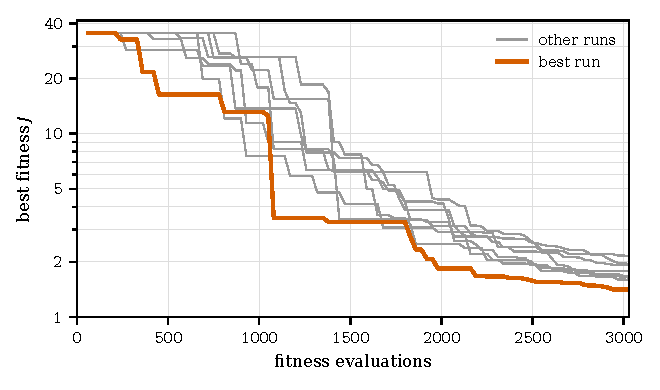
\includegraphics[width=\textwidth]{figures/fig_convergence.pdf}
\caption{(a) Best $J_W$ against cost evaluations for the eight runs, and their median.
(b) Ablation: final $J_T$ of four variants on seeds 1--4 (Sect.~\ref{sec:ablation}).}
\label{fig:convergence}
\end{figure}

\subsection{Tracking Performance}

Table~\ref{tab:comparison} compares FOPSO-GWO-FOPID with the two baselines, and
Figs.~\ref{fig:step} and~\ref{fig:sine} show the responses joint by joint.

\begin{itemize}
\item \textbf{Step.} The tuned controller lowers the mean overshoot from 51.1\,\% (PID) and
  29.2\,\% (FOPID) to 13.6\,\%. The adjustment time falls to 1.35\,s and the peak time to
  1.11\,s. Measured from the step instant, these times fall by 76\,\% and 75\,\% against the
  PID, and by 63\,\% and 68\,\% against the FOPID.
\item \textbf{Sinusoid.} The MSE falls by 91\,\% and 77\,\%.
\item \textbf{ITAE.} Both ITAEs fall by 45--73\,\%.
\end{itemize}

\begin{table}[t]
\caption{Joint-averaged performance of the baselines and the tuned controller, and the
relative change achieved by FOPSO-GWO-FOPID (negative is better)}
\label{tab:comparison}
\centering
\small
\setlength{\tabcolsep}{2.5pt}
\begin{tabular}{lrrrrr}
\toprule
Metric & PID & FOPID & \shortstack{FOPSO-GWO-\\FOPID} & vs PID & vs FOPID\\
\midrule
Overshoot $\sigma$ (\%)         & 51.1 & 29.2 & 13.6 & $-73.3\,\%$ & $-53.4\,\%$\\
Adjustment time $t_s$ (s)       & 2.49 & 1.95 & 1.35 & $-45.8\,\%$ & $-30.6\,\%$\\
Peak time $t_p$ (s)             & 1.45 & 1.35 & 1.11 & $-23.5\,\%$ & $-17.8\,\%$\\
Sine $\MSE$ (rad$^2$)           & $2.12\!\times\!10^{-2}$ & $8.29\!\times\!10^{-3}$ & $1.88\!\times\!10^{-3}$ & $-91.2\,\%$ & $-77.4\,\%$\\
Sine $\Sigma|\tau|$ (N\,m)      & $3.50\!\times\!10^{4}$ & $2.41\!\times\!10^{4}$ & $9.61\!\times\!10^{3}$ & $-72.5\,\%$ & $-60.2\,\%$\\
$\ITAE$, step                   & 4.34 & 2.16 & 1.19 & $-72.6\,\%$ & $-45.1\,\%$\\
$\ITAE$, sine                   & 5.81 & 4.74 & 1.72 & $-70.4\,\%$ & $-63.7\,\%$\\
\bottomrule
\end{tabular}
\end{table}

\begin{figure}[t]
\centering
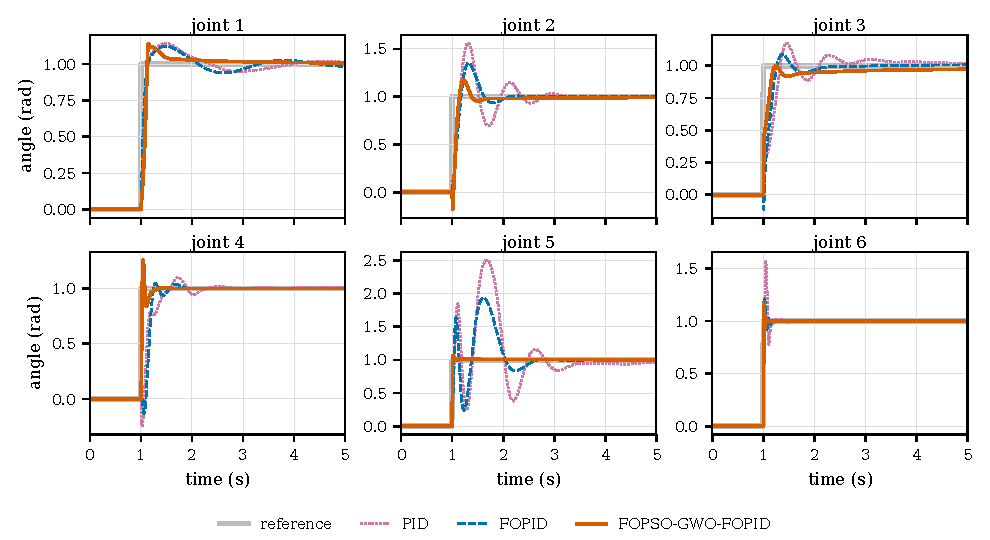
\includegraphics[width=\textwidth]{figures/fig_step.pdf}
\caption{Step responses of the six joints (1\,rad at $t = 1$\,s).}
\label{fig:step}
\end{figure}

\begin{figure}[t]
\centering
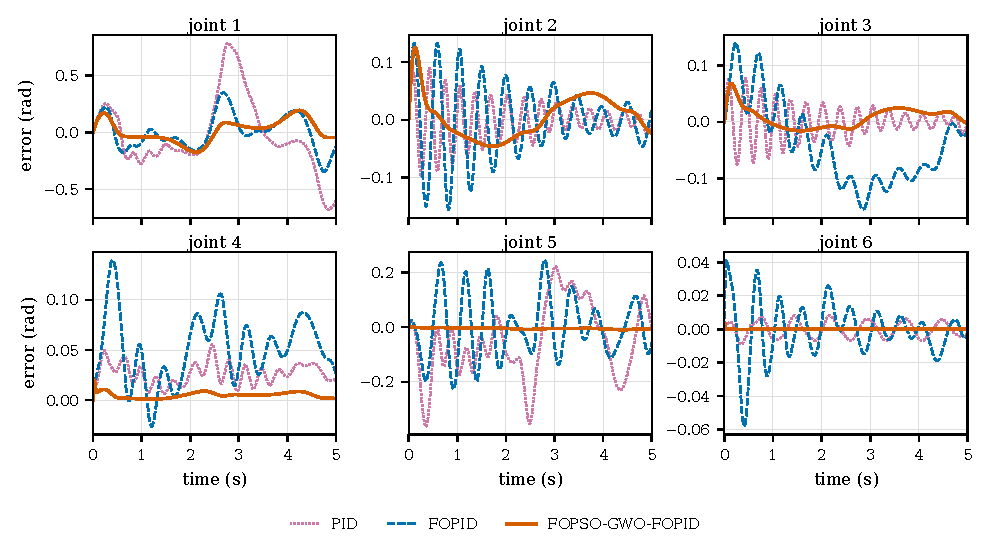
\includegraphics[width=\textwidth]{figures/fig_sine_error.pdf}
\caption{Tracking error $e_j = q_{r,j} - q_j$ for the sinusoidal reference
$q_{r,j} = \sin(1.5\,t)$\,rad.}
\label{fig:sine}
\end{figure}

The averages hide differences between the joints (Table~\ref{tab:perjoint}).
\begin{itemize}
\item \textbf{Largest gains: joints 2, 5 and 6.} The overshoot of joint 5 falls from
  150.2\,\% (PID) and 93.5\,\% (FOPID) to 6.7\,\%. Its sinusoidal MSE falls by more than
  two orders of magnitude.
\item \textbf{Joint 4 is worse.} Its overshoot rises to 25.7\,\%, against 10.0\,\% and
  4.3\,\%. It still stays within the 33.1\,\% limit.
\item \textbf{Joint 3 is overdamped.} It hardly overshoots (0.1\,\%), but settles in 2.07\,s,
  slower than with the FOPID (1.87\,s).
\item \textbf{Joint 1 hardly changes.} Its overshoot (14.3\,\%) is close to that of both
  baselines, and it keeps the largest sinusoidal error of all joints (Fig.~\ref{fig:sine}).
\end{itemize}
These trade-offs follow from the objective, which scores joint averages and limits each joint
only through the caps.

Table~\ref{tab:gains} lists the tuned parameters. Some of them lie at or near the bounds of
the search box: $\lambda_6 = 0.050$, and $K_{d,2} = 989$ against an upper bound of 1000. A
wider box might therefore allow further improvement.

\begin{table}[t]
\caption{Per-joint step overshoot, adjustment time and peak time, and sinusoidal MSE
(``Tuned'': FOPSO-GWO-FOPID)}
\label{tab:perjoint}
\centering
\footnotesize
\setlength{\tabcolsep}{3pt}
\begin{tabular}{llrrrrrr}
\toprule
Metric & Controller & J1 & J2 & J3 & J4 & J5 & J6\\
\midrule
\multirow{3}{*}{$\sigma$ (\%)} & PID   & 14.5 & 56.0 & 17.5 & 10.0 & 150.2 & 58.1\\
                               & FOPID & 12.4 & 35.1 & 8.8  & 4.3  & 93.5  & 21.1\\
                               & Tuned & 14.3 & 17.6 & 0.1 & 25.7 & 6.7 & 17.3\\
\midrule
\multirow{3}{*}{$t_s$ (s)}     & PID   & 1.99 & 2.64 & 2.47 & 2.07 & 4.66 & 1.14\\
                               & FOPID & 2.85 & 1.90 & 1.87 & 1.48 & 2.52 & 1.08\\
                               & Tuned & 1.46 & 1.34 & 2.07 & 1.18 & 1.03 & 1.03\\
\midrule
\multirow{3}{*}{$t_p$ (s)}     & PID   & 1.49 & 1.31 & 1.46 & 1.73 & 1.68 & 1.05\\
                               & FOPID & 1.49 & 1.32 & 1.37 & 1.29 & 1.61 & 1.03\\
                               & Tuned & 1.15 & 1.22 & 1.24 & 1.04 & 1.01 & 1.01\\
\midrule
\multirow{3}{*}{$\MSE$ (rad$^2$)} & PID & 1.0e$-$1 & 1.2e$-$3 & 8.4e$-$4 & 8.2e$-$4 & 2.1e$-$2 & 2.2e$-$5\\
                               & FOPID & 2.3e$-$2 & 3.7e$-$3 & 6.7e$-$3 & 3.8e$-$3 & 1.2e$-$2 & 2.7e$-$4\\
                               & Tuned & 9.4e$-$3 & 1.4e$-$3 & 4.0e$-$4 & 3.4e$-$5 & 3.3e$-$5 & 3.0e$-$8\\
\bottomrule
\end{tabular}
\end{table}

\begin{table}[t]
\caption{Parameters of FOPSO-GWO-FOPID (one set for both scenarios)}
\label{tab:gains}
\centering
\begin{tabular}{lrrrrrr}
\toprule
 & J1 & J2 & J3 & J4 & J5 & J6\\
\midrule
$K_p$     & 110.7 & 0.2054 & 0.03346 & 590.0 & 33.96 & 3393\\
$K_i$     & 42.81 & 132.5 & 0.7265 & 43.96 & 4.420 & $4.329 \times 10^{-4}$\\
$K_d$     & 156.1 & 989.1 & 890.0 & 9.623 & 171.5 & 0.3650\\
$\lambda$ & 1.534 & 0.07579 & 1.377 & 0.07649 & 0.5251 & 0.05009\\
$\mu$     & 0.8239 & 0.5172 & 0.5289 & 0.9728 & 0.7322 & 1.637\\
\bottomrule
\end{tabular}
\end{table}

\subsection{Control Effort and the Role of the Objective}
\label{sec:effort}

Table~\ref{tab:effort} reports the torque at the 1\,kHz control rate. Peaks are the largest
over the joints; sums and total variations are averaged over the joints.

FOPSO-GWO-FOPID improves several effort measures:
\begin{itemize}
\item The derivative kick falls from about $2.2 \times 10^5$\,N\,m to
  $4.6 \times 10^4$\,N\,m, a 79\,\% reduction.
\item The peak torque of the sinusoidal run falls by 53\,\% and 20\,\% against the PID and
  FOPID.
\item The total variation of the sinusoidal torque falls by 91\,\% and 80\,\%.
\end{itemize}
Two step-run measures are not better:
\begin{itemize}
\item The peak torque after the kick is about that of the PID (1517 against 1503\,N\,m).
\item The total variation of the step torque is 45\,\% higher than for either baseline.
\end{itemize}
Perfectly tracking the sinusoid requires $\Sigma|\tau| = 7.40 \times 10^{3}$\,N\,m by inverse
dynamics; the tuned controller uses 1.30 times that. The 60--73\,\% reduction of
$\Sigma|\tau|$ in Table~\ref{tab:comparison} should be read with care. The baseline gains were
fitted to the torque sums \emph{reported} in~\cite{jiang2025}. PID and FOPID gains fitted to
the published response curves instead need only about $1.0 \times 10^{4}$\,N\,m.

\begin{table}[t]
\caption{Control effort at the 1\,kHz control rate (N\,m). The last column is the best run
of FOPSO-GWO tuned for $J_{\ITAE}$ alone}
\label{tab:effort}
\centering
\small
\setlength{\tabcolsep}{4pt}
\begin{tabular}{lrrrr}
\toprule
 & PID & FOPID & \shortstack{FOPSO-GWO-\\FOPID} & \shortstack{ITAE-\\tuned}\\
\midrule
Kick peak (first 50\,ms) & $2.16 \times 10^{5}$ & $2.28 \times 10^{5}$ & $4.64 \times 10^{4}$ & $6.48 \times 10^{5}$\\
Step peak after the kick                & 1503 & 3114 & 1517 & 2797\\
Sine peak                               & 879.2 & 516.7 & 412.9 & 1417\\
Step $\Sigma|\tau|$ after the kick      & $1.22 \times 10^{4}$ & 8928 & 8480 & 9012\\
Sine $\Sigma|\tau|$                     & $3.50 \times 10^{4}$ & $2.41 \times 10^{4}$ & 9610 & 9512\\
Step total variation                    & 1054 & 1072 & 1552 & 1665\\
Sine total variation                    & 6307 & 2940 & 596.6 & 1339\\
Limits exceeded (of 18)          & -- & -- & 0 & 7\\
\bottomrule
\end{tabular}
\end{table}

The last column of Table~\ref{tab:effort} shows what the effort terms and the limits buy. It
is the best of the eight FOPSO-GWO runs tuned for $J_{\ITAE}$ alone.
\begin{itemize}
\item \textbf{Tracking is better.} Its step ITAE is 0.248 against 1.188, and its sinusoidal
  MSE is $3.1 \times 10^{-4}$ against $1.9 \times 10^{-3}$\,rad$^2$.
\item \textbf{Effort is far worse.} Its derivative kick reaches $6.5 \times 10^5$\,N\,m,
  14 times that of FOPSO-GWO-FOPID. Its peak sinusoidal torque is 3.4 times higher.
\item \textbf{It is not admissible.} It exceeds 7 of the 18 torque limits: the kick limit on
  two joints, up to 14.9 times, and the step limit on five joints, up to 1.9 times.
\end{itemize}
The whole-controller objective gives up some tracking to stay within limits that an actuator
can meet.

\subsection{Ablation}
\label{sec:ablation}

Table~\ref{tab:ablation} and Fig.~\ref{fig:convergence}(b) compare FOPSO-GWO with variants
that each change one design choice, all under the same budget and initial swarms.
\begin{itemize}
\item \textbf{Grey-wolf term.} Removing it, which leaves a fractional-order PSO with
  $c_1 = c_2 = 2$, raises the mean $J_T$ from 0.346 to 0.469 (+35\,\%).
\item \textbf{Coefficients.} Adding the wolf term on top of $c_1 = c_2 = 2$ is worse still
  (0.634), because the swarm becomes erratic. With $c = 1/1/1$ and a decreasing order, it
  collapses early (0.425).
\item \textbf{Consistency under $J_W$.} The final settings lower the median of $J_W$ from
  1.951 to 1.718 and its worst run from 2.694 to 2.160.
\item \textbf{Where the initial settings win.} Their single best $J_W$ run is lower (1.076
  against 1.416). Under $J_{\ITAE}$ their mean is marginally lower (0.116 against 0.123 on
  seeds 1--4).
\end{itemize}
The final settings therefore trade some peak performance for consistency, which is the
property that matters when only a few runs can be afforded.

\begin{table}[t]
\caption{Ablation: mean final cost of FOPSO-GWO variants under the same budget and initial
swarms ($J_T$ and $J_{\ITAE}$: seeds 1--4; $J_W$: seeds 1--8)}
\label{tab:ablation}
\centering
\begin{tabular}{lllrrr}
\toprule
Variant & $c_1/c_2/c_3$ & order $a$ & $J_T$ & $J_W$ & $J_{\ITAE}$\\
\midrule
Fractional-order PSO (no grey-wolf term) & 2/2/0 & $0.9 \to 0.4$ & 0.469 & -- & --\\
Wolf term added on top                   & 2/2/2 & $0.9 \to 0.4$ & 0.634 & -- & --\\
Initial settings                          & 1/1/1 & $0.9 \to 0.4$ & 0.425 & 1.929 & 0.116\\
\textbf{FOPSO-GWO (final)}               & 1.5/1.5/1 & 0.9 & \textbf{0.346} & \textbf{1.764} & 0.123\\
\bottomrule
\end{tabular}
\end{table}

% =====================================================================
\section{Discussion and Limitations}
\label{sec:discussion}

The results support a narrower claim than ``FOPSO-GWO is a better optimiser''. Tuning the
30 FOPID parameters with the whole-controller objective yields a controller that clearly
outperforms the reproduced PID and FOPID baselines, while respecting per-joint torque limits
that an ITAE-tuned controller violates. Several limitations qualify this result:
\begin{itemize}
\item \textbf{Baselines.} They reproduce published results; they were not re-tuned with the
  same objective and budget. The comparison therefore measures the benefit of tuning with
  $J_W$, not the merit of FOPSO-GWO relative to other optimisers. Such a claim requires a
  comparison with other tuning algorithms under identical budgets, initial populations and
  objectives, and no algorithm can be expected to win on every
  problem~\cite{wolpert1997}.
\item \textbf{Statistics.} Eight runs per objective are enough to show the spread of the
  method, but not to resolve small differences between variants. Under $J_{\ITAE}$ the
  seed-to-seed spread is as large as the differences between settings.
\item \textbf{Model.} The arm is simulated with nominal parameters, without gravity, joint
  friction, actuator dynamics, sensor noise or torque saturation, and only for the two
  reference signals of the benchmark. Robustness to parameter errors and experiments on
  hardware remain to be shown.
\item \textbf{Limits.} The tuned controller operates close to several limits. In practice
  the limits should be set with a margin below the actuator ratings.
\end{itemize}

The objective is close to a sum of per-joint contributions, because each joint's controller
mostly shapes its own response. This suggests decomposing the search by joint as a direction
for future work.

% =====================================================================
\section{Conclusion}
\label{sec:conclusion}

This paper tuned the six FOPID controllers of a 6-DOF robotic arm with FOPSO-GWO, a
fractional-order particle swarm optimiser with a grey-wolf term. The whole-controller objective balances step and
sinusoidal tracking against control effort under 24 per-joint limits. Compared with PID and
FOPID baselines that reproduce published results within 6.5\,\%, the tuned controller lowers
the mean overshoot by 73\,\% and 53\,\%, the settling time by 46\,\% and 31\,\%, the
sinusoidal MSE by 91\,\% and 77\,\% and the derivative-kick torque by 79\,\%. All eight
independent runs satisfied every limit. The same optimiser with an ITAE-only objective tracks
better but breaks 7 of the 18 torque limits, which shows that the effort terms and limits are
essential for an applicable controller. Future work will compare FOPSO-GWO with other tuning
algorithms under identical conditions, add gravity, friction and parameter uncertainty, and
validate the controller on hardware.

% TODO: acknowledgements, data and code availability statement (after review)

\bibliographystyle{spmpsci}
\bibliography{references}

\end{document}
